\section{Etapas de operação}


As etapas de operação dos Star Tracks, em geral, seguem a estrutura apresentada na Figura ~\ref{fig:etapas_star_trackers}.


\begin{figure}[H]
	\centering
	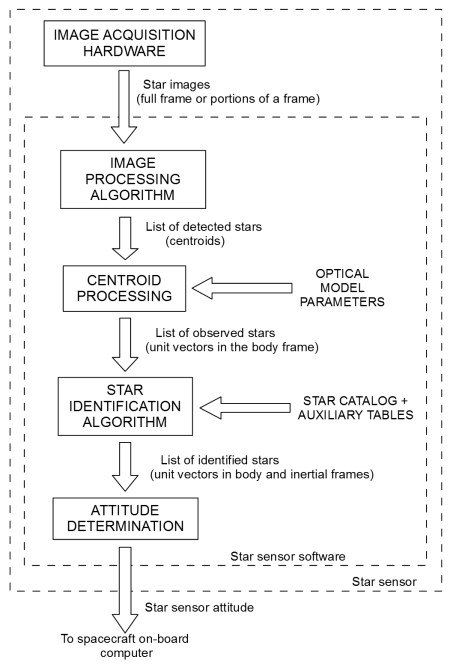
\includegraphics[width=.6\columnwidth]{images/etapas.jpg}
	\caption{Etapas de funcionamento de um Star Tracker. Fonte: ~\cite[]{Fialho}}
	\label{fig:etapas_star_trackers}
\end{figure}

A primeira etapa de operação, consiste  na aquisição da imagem a ser utilizada, para tal é utilizado um CCD acoplado a um conjunto de lentes. A escolha desse componentes deve levar em conta uma série de parâmetros, tais como: abertura do campo visual, precisão, volume, peso e outros a variar com a  missão do cubesat ~\cite[]{Carvalho}. Neste projeto a aquisição de imagens será feita com uma \textit{webcam}.

O algoritmo de processamento juntamente com processamento de centroide, são responsáveis por localizar cada uma das estrelas e determinar sua localização e intensidade.

O algoritmo de identificação de estrelas é responsável por fazer a relação entre as estrelas identificadas na observação e as estrelas contidas no banco de dados. A identificação de uma estrela envolve a análise das relações entre as diversas estrelas observadas, para tal utiliza-se algoritmos como de  \textit{Planar Triangles} ~\cite[]{Cole}.

Por fim, é determinada a atitude do cubesat, que pode ser feita utilizando ângulos de Euler ou quaternions.

Para avaliar os algoritmos desenvolvidos, foi implementado um simulador estrelar, seguindo o método demonstrado por Tappe ~\cite[]{Tappe}. 
Por fim, foram realizados testes com imagens reais obtidas por \textit{webcams}  ou câmeras de celulares.

